\documentclass{article}
\usepackage[utf8]{inputenc}


\usepackage[margin=1.04 in]{geometry}
\usepackage[T1]{fontenc}
\usepackage{mathtools}   % loads »amsmath«
\usepackage{amssymb}
\usepackage{amsfonts}
\usepackage{amsmath}
\usepackage{amsthm}
\usepackage{xcolor}
\usepackage{cancel}
%\usepackage{graphics}
\usepackage{graphicx}
%others
\usepackage{enumerate}
\usepackage{subcaption}



\usepackage{apacite}
\usepackage[round]{natbib}
%\bibliographystyle{plainnat}
\bibliographystyle{apacite}

\DeclarePairedDelimiter{\ceil}{\lceil}{\rceil}

\setlength{\parskip}{0.6em}
\usepackage{setspace}
\spacing{1.2}


\newtheorem{defin}{Definition.}
\newtheorem{teo}{Theorem. }
\newtheorem{lema}{Lemma. }
\newtheorem{coro}{Corolary. }
\newtheorem{prop}{Proposition. }
\theoremstyle{definition}
\newtheorem{examp}{Example. }
\newtheorem{problem}{}


\title{Problem Set 4}
\author{Giselle Labrador Badía}
\date{November 2021}

\begin{document}

\maketitle

This Problem Set uses data from \cite{jia2008happens}
\section*{Question 1}

The table below shows estimates for two different specifications of the model, both for Walmart presence and Kmart presence. We run 4 probit regressions and obtain significant coefficients for most of our market characteristic variables. The first one is using the following market characteristics: $log(population)$, \% of urban population, a Midwest dummy, a south dummy, and the Kmart or Walmart dummy respectively. The second setup is adding the number of small stores in every market. 
\begin{table}[h]
\begin{center}
\begin{tabular}{l c c c c}
\hline
 & kmart & kmart & wal & wal \\
\hline
(Intercept)     & $-6.60^{***}$ & $-6.61^{***}$ & $-6.75^{***}$ & $-6.64^{***}$ \\
                & $(0.29)$      & $(0.29)$      & $(0.36)$      & $(0.36)$      \\
log\_pop        & $1.64^{***}$  & $1.64^{***}$  & $1.56^{***}$  & $1.46^{***}$  \\
                & $(0.08)$      & $(0.09)$      & $(0.10)$      & $(0.10)$      \\
perc\_urb\_pop  & $1.82^{***}$  & $1.82^{***}$  & $1.73^{***}$  & $1.86^{***}$  \\
                & $(0.17)$      & $(0.17)$      & $(0.21)$      & $(0.21)$      \\
midwest\_dummy  & $0.98^{***}$  & $0.98^{***}$  & $0.57^{***}$  & $0.60^{***}$  \\
                & $(0.13)$      & $(0.13)$      & $(0.14)$      & $(0.14)$      \\
south\_dummy    & $1.30^{***}$  & $1.30^{***}$  & $0.09$        & $0.04$        \\
                & $(0.13)$      & $(0.13)$      & $(0.14)$      & $(0.14)$      \\
kmart\_dummy    & $-0.48^{***}$ & $-0.48^{***}$ &               &               \\
                & $(0.10)$      & $(0.10)$      &               &               \\
small\_stor     &               & $-0.00$       &               & $0.04^{*}$    \\
                &               & $(0.02)$      &               & $(0.02)$      \\
walmart\_dummy &               &               & $-0.33^{***}$ & $-0.33^{***}$ \\
                &               &               & $(0.10)$      & $(0.10)$      \\
\hline
AIC             & $1755.77$     & $1757.76$     & $1318.49$     & $1314.63$     \\
BIC             & $1789.57$     & $1797.19$     & $1352.29$     & $1354.06$     \\
Log Likelihood  & $-871.88$     & $-871.88$     & $-653.25$     & $-650.31$     \\
Deviance        & $1743.77$     & $1743.76$     & $1306.49$     & $1300.63$     \\
Num. obs.       & $2065$        & $2065$        & $2065$        & $2065$        \\
\hline
\multicolumn{5}{l}{\scriptsize{$^{***}p<0.001$; $^{**}p<0.01$; $^{*}p<0.05$}}
\end{tabular}
\caption{Regressions results for first question}
\label{tab:1}
\end{center}
\end{table}

To interpret these coefficients easily, we plot the average marginal effect for the Walmart regression. For instance, these regressions suggest that Kmart's presence decrease by approximately 11 \% with Walmart's entry. 




\begin{figure}[h]
\centering
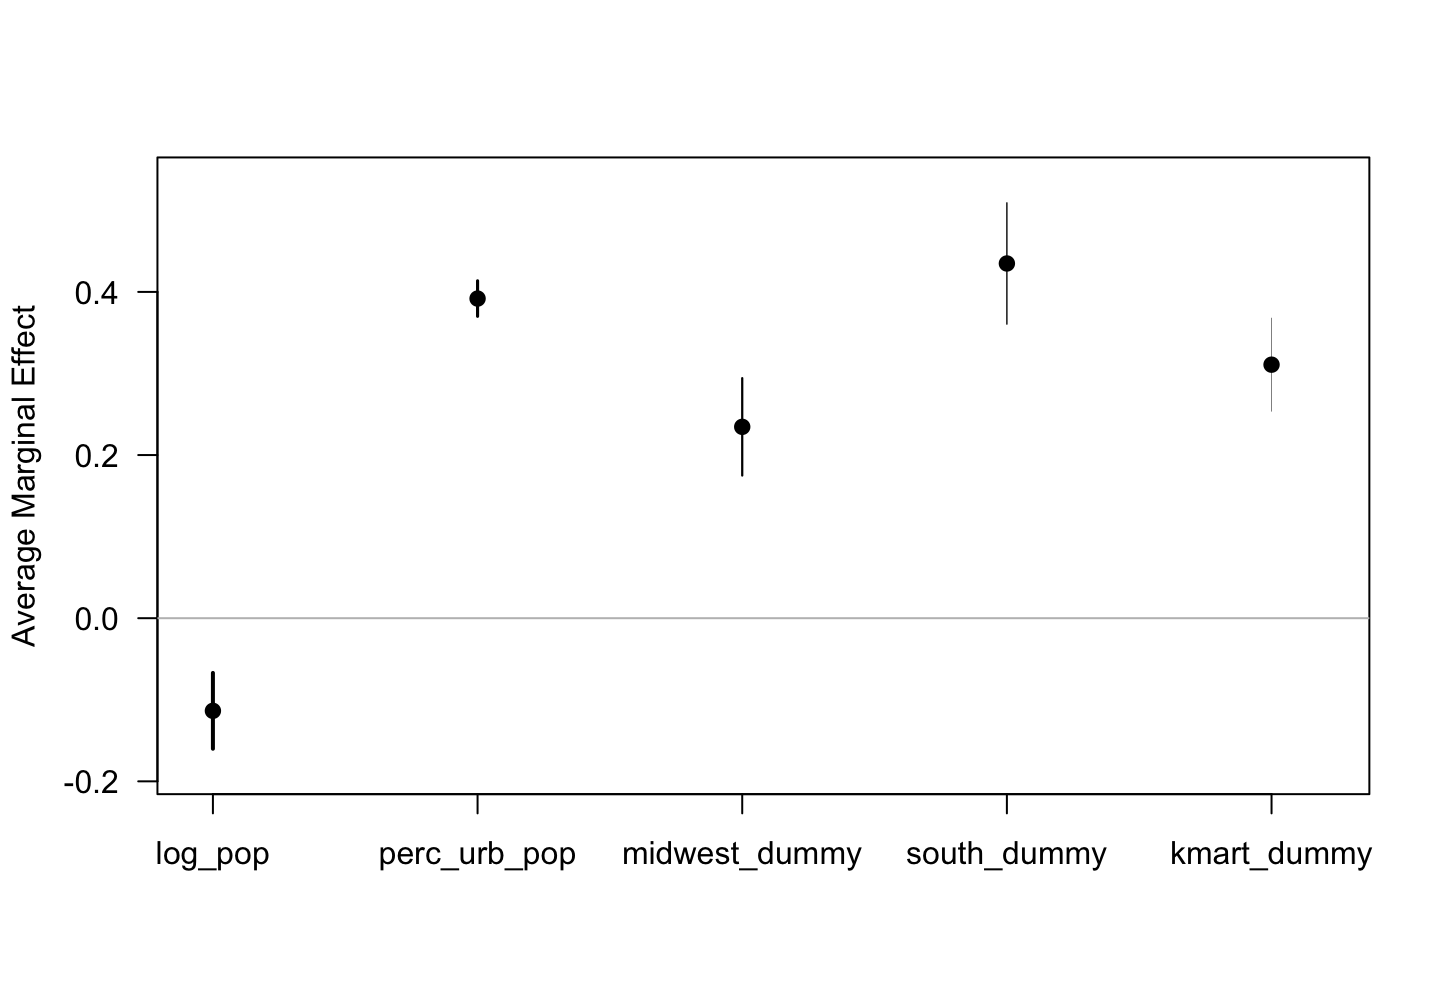
\includegraphics[width=0.6\textwidth]{imgs/ave_1_w.png}
\caption{AME for Walmart probit regression. (Kmart label and log population marginal effects are interchanged)}
\end{figure}

One weakness of this model is that we want to model strategic entry, and we don't have dynamic data. Hence, we cannot tell whether Walmart or Kmart are entering the market because the other firm entered first.  We also are missing some key market-level characteristics such as household income, and demographics. 

\section*{Question 2}

To deal with endogeneity we use the instrument distance to Benton, Arkansas. This is because this is where Walmart headquarters are located, so this variable should impact the expansion of Walmart. That is, Walmart entry can be determined by the closeness with this county since entry to close markets is less costly than entry to very distant markets. Discussing the exogeneity of the instrument, it is not completely clear that this should not affect the rivals' decisions of entering a market. 


\begin{table}[ht]
\centering
\begin{tabular}{rrrrr}
  \hline
 & Coef & S.E. & t-stat & p-val \\ 
  \hline
Intercep & -10.96 & 0.78 & -14.13 & 0.00 \\ 
  log\_pop & 3.06 & 0.26 & 11.88 & 0.00 \\ 
  perc\_urb\_pop & 3.33 & 0.36 & 9.33 & 0.00 \\ 
  midwest\_dummy & 1.33 & 0.22 & 6.10 & 0.00 \\ 
  south\_dummy & 1.12 & 0.24 & 4.64 & 0.00 \\ 
  walmart\_dummy & -3.90 & 0.56 & -6.96 & 0.00 \\ 
   \hline
\end{tabular}
\end{table}

First, we attempt an iv-probit regression of Kmart on Walmart and other market characteristics. Walmart is treated as endogenous, using distance to Benton as an instrument. Below, we display a table with the results of the IV-probit regression. We did not include first stage coefficients for this exercise, but in table 4 (question 4), coefficients for regression of Walmart on Benton distance are displayed on the first column, and the effect and significance of the instrument can be verified. 

We opt for control functions (two-stage residual inclusion) approach to correct for endogeneity.  We choose control functions (CF) because of their advantages such as working for non-invertible models in particular discrete choice models. We implement two specifications,  one with OLS in the first stage and probit in the first stage. We always regress Kmart on Walmart using both the endogenous variable and the residual. 



\begin{table}[h]
\begin{center}
\begin{tabular}{l c c}
\hline
 & CF w/ OLS & CF w/ probit \\
\hline
(Intercept)       & $-16.90^{***}$ & $-15.31^{***}$ \\
                  & $(0.89)$       & $(0.80)$       \\
log\_pop          & $5.12^{***}$   & $4.52^{***}$   \\
                  & $(0.30)$       & $(0.26)$       \\
perc\_urb\_pop    & $5.56^{***}$   & $4.92^{***}$   \\
                  & $(0.38)$       & $(0.34)$       \\
midwest\_dummy    & $2.32^{***}$   & $2.14^{***}$   \\
                  & $(0.20)$       & $(0.19)$       \\
south\_dummy      & $2.44^{***}$   & $2.19^{***}$   \\
                  & $(0.22)$       & $(0.21)$       \\
walmart\_dummy   & $-8.62^{***}$  & $-7.56^{***}$  \\
                  & $(0.63)$       & $(0.55)$       \\
res\_wal         & $8.62^{***}$   & $3.08^{***}$   \\
                  & $(0.64)$       & $(0.23)$       \\
\hline
AIC               & $1048.16$      & $1055.96$      \\
BIC               & $1087.59$      & $1095.39$      \\
Log Likelihood    & $-517.08$      & $-520.98$      \\
Deviance          & $1034.16$      & $1041.96$      \\
Num. obs.         & $2065$         & $2065$         \\
\hline
\multicolumn{3}{l}{\scriptsize{$^{***}p<0.001$; $^{**}p<0.01$; $^{*}p<0.05$}}
\end{tabular}
\caption{Control function regressions,  second question}
\label{tab:1}
\end{center}
\end{table}

Comparing these results with question 1, we see that not accounting for endogeneity underestimates the size of the impact of Walmart on Kmart's presence. Moreover, using control function (CF) approach, these coefficients are bigger. It is better to use OLS in the first stage since with probit the residuals are non-linear.  

\section*{Question 3}

We conduct ordered probit regressions for two dependant variables: number of large competitors ($L = 1(Kmart) + 1(Walmart)$ could take values 0,1, and 2 ) and total number of stores ($L = 1(Kmart) + 1(Walmart) + #small\_stores$) (Table 4). The first model seems to fit better (according to AIC and BIC). We omitted the ordered probit coefficients since this made the table long and it was not clear how to interpret these coefficients.

\begin{table}[h]
\begin{center}
\begin{tabular}{l c c}
\hline
 & \#Large Stores & \#Total Stores \\
\hline
log\_pop       & $1.79^{***}$ & $1.46^{***}$ \\
               & $(0.07)$     & $(0.05)$     \\
perc\_urb\_pop & $1.97^{***}$ & $-0.21$      \\
               & $(0.15)$     & $(0.11)$     \\
midwest\_dummy & $0.89^{***}$ & $-0.10$      \\
               & $(0.12)$     & $(0.09)$     \\
south\_dummy   & $0.89^{***}$ & $0.53^{***}$ \\
               & $(0.11)$     & $(0.09)$     \\
\hline
AIC            & $2522.76$    & $8237.27$    \\
BIC            & $2556.56$    & $8333.03$    \\
Log Likelihood & $-1255.38$   & $-4101.64$   \\
Deviance       & $2510.76$    & $8203.27$    \\
Num. obs.      & $2065$       & $2065$       \\
\hline
\multicolumn{3}{l}{\scriptsize{$^{***}p<0.001$; $^{**}p<0.01$; $^{*}p<0.05$}}
\end{tabular}
\caption{Regressions results for third question (TABLE II)}
\label{tab:1}
\end{center}
\end{table}



The obvious weakness of this model is that firm size is not comparable. Walmart is a huge player, the biggest employer in the United States, whereas Kmart is a smaller and not as profitable chain. Moreover, the small stores are added up to Walmart and Kmart entry as equals. Firms are not homogeneous, so maybe using a model with appropriate weights for every company will be more adequate. 



\section*{Question 4}

These questions follow the methodology of \cite{bajari2010estimating}. We proceed with a two-stage regression to estimate the static game. In the first stage, we estimate the regressions Walmart and Kmart probit regressions, using the instrument proposed in 2. in the Walmart case. In the second stage, we use the predicted values from the regression and run probit regressions for Kmart and Probit respectively. The variables that have the $pr$ subscripts mean that these are predictions from the first stage. 

\begin{figure}[h]
\centering
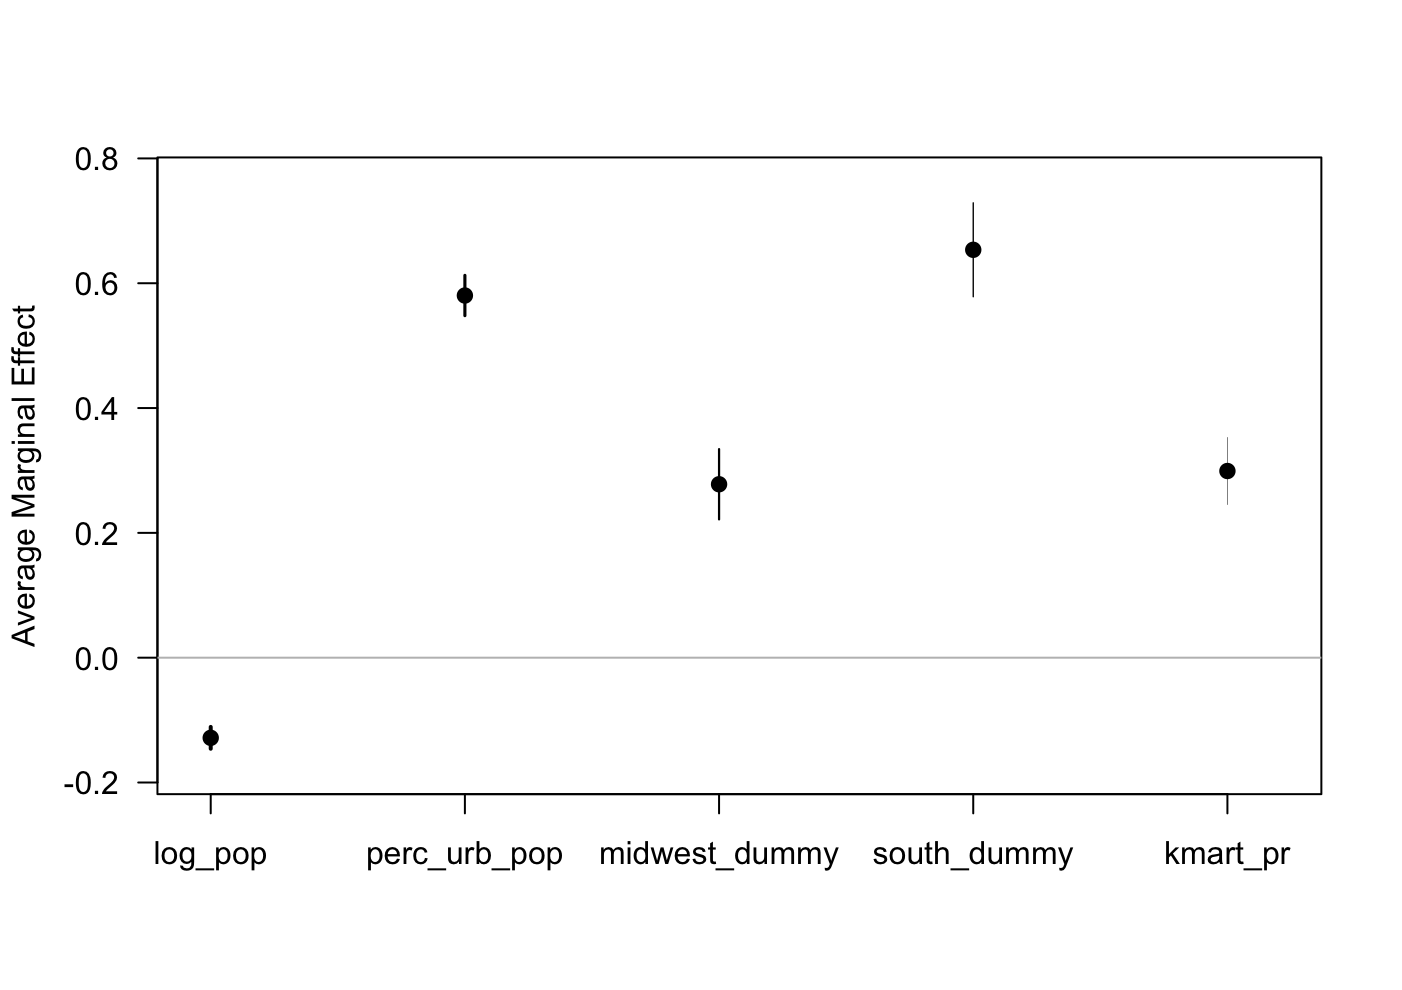
\includegraphics[width=0.6\textwidth]{imgs/ave_4_w.png}
\caption{AME for walmart probit regression, question 4. (Kmart label and log population marginal effects are interchanged)}. 
\end{figure}

\begin{table}[h]
\begin{center}
\begin{tabular}{l c c c c}
\hline
 & I St Wal & II St Kmart & I St Kmart & II St Wal \\
\hline
(Intercept)       & $-0.53$       & $-16.90^{***}$ & $-6.75^{***}$ & $-11.45^{***}$ \\
                  & $(0.56)$      & $(0.89)$       & $(0.36)$      & $(0.54)$       \\
log\_pop          & $1.78^{***}$  & $5.12^{***}$   & $1.56^{***}$  & $2.69^{***}$   \\
                  & $(0.08)$      & $(0.30)$       & $(0.10)$      & $(0.13)$       \\
perc\_urb\_pop    & $1.93^{***}$  & $5.56^{***}$   & $1.73^{***}$  & $3.03^{***}$   \\
                  & $(0.18)$      & $(0.38)$       & $(0.21)$      & $(0.21)$       \\
midwest\_dummy    & $0.15$        & $2.32^{***}$   & $0.57^{***}$  & $1.29^{***}$   \\
                  & $(0.15)$      & $(0.20)$       & $(0.14)$      & $(0.14)$       \\
south\_dummy      & $0.53^{***}$  & $2.44^{***}$   & $0.09$        & $1.39^{***}$   \\
                  & $(0.15)$      & $(0.22)$       & $(0.14)$      & $(0.14)$       \\
kmart\_dummy      & $-0.30^{**}$  &                &               &                \\
                  & $(0.11)$      &                &               &                \\
log\_dist\_benton & $-0.93^{***}$ &                &               &                \\
                  & $(0.08)$      &                &               &                \\
walmart\_pr      &               & $-8.62^{***}$  &               &                \\
                  &               & $(0.63)$       &               &                \\
walmart\_dummy   &               &                & $-0.33^{***}$ &                \\
                  &               &                & $(0.10)$      &                \\
kmart\_pr         &               &                &               & $-0.60^{***}$  \\
                  &               &                &               & $(0.05)$       \\
\hline
AIC               & $1585.49$     & $1046.16$      & $1318.49$     & $1584.03$      \\
BIC               & $1624.92$     & $1079.95$      & $1352.29$     & $1617.83$      \\
Log Likelihood    & $-785.74$     & $-517.08$      & $-653.25$     & $-786.01$      \\
Deviance          & $1571.49$     & $1034.16$      & $1306.49$     & $1572.03$      \\
Num. obs.         & $2065$        & $2065$         & $2065$        & $2065$         \\
\hline
\multicolumn{5}{l}{\scriptsize{$^{***}p<0.001$; $^{**}p<0.01$; $^{*}p<0.05$}}
\end{tabular}
\caption{Regressions results for forth question (TABLE III)}
\label{tab:1}
\end{center}
\end{table}


To interpret these coefficients easily, we plot the average marginal effect for the second stage Walmart probit regression. As you can see for Walmart the effects obtained are larger using this two-stage process than with the simple regression in question 1. This suggests that firms do engage in strategic behavior, and the evidence is stronger using this method than with simple probit or with iv-probit regression.  Ideally we will run a non-parametric or semi-parametric regression as in \cite{bajari2010estimating}.

To calculate the standard error we use the variance-covariance matrix. We would see entry as endogenous, and use GMM or maybe Two-Stage Least Squared to get the matrices.






\bibliography{references}

\end{document}